\documentclass{article}

% Language setting
% Replace `english' with e.g. `spanish' to change the document language
\usepackage[english]{babel}
% Please add the following required packages to your document preamble:
% \usepackage{booktabs}
% Set page size and margins
% Replace `letterpaper' with `a4paper' for UK/EU standard size
\usepackage[letterpaper,top=2cm,bottom=2cm,left=3cm,right=3cm,marginparwidth=1.75cm]{geometry}

% Useful packages
\usepackage{CJKutf8}
\usepackage{amsmath}
\usepackage{graphicx}
\usepackage[colorlinks=true, allcolors=blue]{hyperref}
\usepackage{booktabs}
\usepackage{tabularx}
\usepackage{sidenotes}

\title{N1 Print Tuning Effect Meta-Analysis}
\author{Alex X. Ye, Kexin Huang, Urs Maurer}

\begin{document}
\maketitle

\begin{abstract}
\end{abstract}
\section{Introduction}
\subsection{The N1 print tuning effect}

In electroencephalography (EEG), the N1 print tuning effect is identified as the greater negativity for L1 words than symbols or unfamiliar words (words that participants do not know of) in the occipito-temporal electrodes and positivity in central fronto-parietal electrodes at around 120-200 ms after the stimulus onset (Maurer et al., 2006; Xue, 2008; Brem et al., 2010; Wang and Maurer, 2020). It is associated with reading expertise since longitudinal studies found increased N1 print tuning effect in children as they acquire reading skills (e.g. association between orthographical and phonological information), %and studies comparing English monolingual speakers and English-Chinese bilingual speakers revealed that N1 print tuning effect only emerges for familiar characters when compared to unfamiliar or pseudofont characters (Maurer \& McCandliss, 2005; Wong et al., 2005). 
\subsection{Research Question and Research Hypotheses}

Previous studies investigating this effect found different results in different time frames. To look into the temporal details, previous studies used two methods to analyze their data: N1 segmentation based on Global Field Power (GFP), and peak latency analysis. By identifying the minima and maxima of the grand average GFP curves, some studies segmented the N1 component into early (minima of N1 onset to peak) and late (peak to minima of N1 offset) parts (Wang and Maurer, 2017; Wang and Maurer, 2020). While early N1 consistently presents the N1 print tuning effect, a study combining EEG and fMRI reported more pronounced difference between word and symbol conditions (Brem, 2006), and another study reported weaker effect compared to that occurred in early N1 (Eberhard-Moscicka at al., 2016). Peak latency analyses also had mixed findings: some studies found a consistent earlier peak for word condition and later peak for control condition (Shirahama, 2004; Wang and Maurer, 2017; Wang and Maurer, 2020), other studies did not find a significant difference between the two (Eulitz, 2000; Eberhard-Moscicka et al., 2016).
 
A further look at previous studies suggested that for studies that did not find significant latency difference (Eulitz, 2000; Eberhard-Moscicka et al., 2016),  they used false-fonts instead of symbols in previous studies and kept using alphabetic words in the word condition. As false-fonts might share more visual similarity with real words when compared with symbols, the findings might suggest that visual similarity between word and control conditions could potentially influence the N1 print tuning effect.

This influence, however, might also be due to the writing system, as studies that found inconsistent results used word from alphabetic writing system (Eulitz, 2000; Brem, 2006; Eberhard-Moscicka et al., 2016), while studies using stimuli in logo-graphic system found consistent difference in early and late N1 (Wang and Maurer, 2017; Wang and Maurer, 2020).

It would thus be interesting to test the influence of visual similarity on the N1 print tuning effect during the early and late stage of N1. % To measure the effect of visual similarity on N1 print tuning effect in different stages of N1, this study plans to combine data from previous studies in different writing systems and conduct a meta-analysis. 

This study hypothesizes that: 1) Among the selected studies, there is a difference in the processing time window of N1 print tuning effect, and 2) visual similarity shows a moderation effect on such a difference. If the visual similarity does not show a significant moderation effect, an alternative hypothesis is that writing system might serve as a moderator.
\section{Methods}

Combining the EEG data analysis and image analysis of stimuli used in experiments, this study first conduct a meta-analysis on the EEG data collected from previous studies to test hypothesis 1. After that, an image analysis to quantify the visual similarity of stimuli used in the experiments is conducted. In this analysis, the physical features of stimuli are quantified as 5 parameters: perimetric complexity (PC), object number, disconnected stroke, stroke sum, and junctions, which together indicate visual complexity. The visual similarity is defined as the difference between the visual complexity of the stimuli, and a smaller difference between conditions indicates greater visual similarity. This visual similarity index is later added into the meta-analysis as an factor to test whether it shows moderation effect.
\subsection{Meta-Analysis}

This meta-analysis is based on the EEG data collected from 7 previous studies. Specifically, these studies used German, English, Chinese as stimuli for the familiar word condition, while symbols, false-fonts and Korean were used for unfamiliar word or symbol condition. We selected these studies because we had access to the data through Dr. Urs Maurer. @STATEMENT OF INTERESTS?@

The data was preprocessed separately for each study. After artifact rejection, offline filtering, baseline correction, selecting target epoch, and ICA (Maurer \& Brandeis et al., 2005; Maurer \& McCandliss, 2005; Maurer \& McCandliss, 2008; Eberhard-Moscicka et al., 2016; Wang \& Maurer, 2017), the GFP was calculated for each condition within each study individually. The N1 segmentation was conducted based on the same criteria as previous studies. The raw data collected for this meta-analysis contains the average amplitude within early or late N1 of specific participant in each condition of the same task and different electrodes.

The raw data was first preprocessed before being coded and used for the final analysis. For each study, this preprocessing involves three steps: 1. Selecting target electrode; 2. Calculating average amplitude across all participants; 3. Calculating the standard deviation of amplitudes of all participants.

As previous studies found that the left hemisphere in temporo-occipital lobe showed the robustest N1 print tuning effect (Maurer et al., 2005; Maurer et al., 2006; Xue, 2008; Brem et al., 2010; Wang and Maurer, 2020), this study limit electrode selection to the left hemisphere. Finally, the electrode in the left hemisphere with largest difference in amplitudes between word and control conditions was selected.
%To find the largest N1 print tuning effect, the amplitudes in the word condition group and that of the control (symbol/false-font/unfamiliar word) condition group was compared with t-test, and the target electrode should be the one with largest difference between two groups and smallest p-value. 

For all studies included, the left occipital-temporal cluster electrodes displayed the robustest difference between word and control condition. Among these studies, the first study used a different EEG system from others. To unify all studies, reference is made to technical document from EGI (Luu \& Ferree, 2005) to help identify which electrodes are located in nearest locations in different systems. For the first study, the electrode showing the robustest N1 print tuning effect is PO9, which is the closest to E64 in the other system. As this electrode also displayed robust N1 print tuning effect in the other studies, we decide to choose PO9 and E64 as target electrodes.
% In the first paper included for this meta-analysis (Maurer et al., 2005), the electrode showing the most robust N1 print tuning effect is PO9 (p < .000), which locates precisely in the target area (left occipito-temporal cluster). However, it is also worth noticing that this study used a different EEG system than the others. To align all studies, the electrode (in the 128-channel system) that is nearest to PO9 of 48-channel system was chosen for the rest of the studies. According to the technical document from EGI (Luu \& Ferree, 2005), this electrode might be E64 since it is closest to P9 but with a 2-centimeter error. Another candidate can be E69 for that it is also close to the position of PO9 but not listed in the document. Still, by comparing the final meta-analysis results from both electrodes, there is no large difference between the effect size of E69 and that of E64. Thus, this study uses the result of E64 for the final analysis.

After selecting the target electrode, the average amplitude across all participants for specific electrode (PO9 or E64), task type (repetition detection or script decision) was calculated for each time window (N1 onset and N1 offset), word condition (word condition and control condition) separately for each study. The standard deviation is calculated in a similar manner.

\subsection{Visual Similarity Analysis}

Based on Chang (2015), where the author used 4 parameters to quantify visual complexity, this study used 5 parameters to measure the visual complexity of stimuli. In addition to number of strokes, disconnected strokes, junctions, and PC, we added object number as 5th parameter. This parameter is added as it offers additional information for visual complexity within smaller parts of a character. 

As Watson (2011) suggested, PC is a shape descriptor that quantifies the complexity of an object's perimeter relative to its area. The image is first loaded using the Python Imaging Library (PIL) and converted to a grayscale representation, then calculated through the following steps:

\textbf{Perimeter Extraction:} Inside the image, the object's perimeter in the image is determined through a series of operations involving the application of the ImageChops module from PIL. %Initially, two sets of offsets are generated: offsets1 and offsets2. Subsequently, the first set of offsets is applied to the original image, resulting in a composite image formed by selecting the darker pixel value from each pair of corresponding pixels in the original and offset images. The perimeter is then obtained by subtracting the composite image from the original image and inverting the resultant image.

\textbf{Ink Area Calculation:} The ink area of the image is computed by inverting the original image, summing the intensities of all pixels, and normalizing the values by dividing them by 255.

\textbf{Perimetric Complexity Calculation:} Based on the calculated perimeter and ink area, the perimetric complexity is derived using the equation \ref{PC_equa}.
\begin{equation}
\label{PC_equa}
    PC = (perimeter ^ 2) / (inkArea * 4 * \pi)
\end{equation}

This method facilitates the quantification of an image's perimetric complexity, serving as a valuable shape descriptor for a variety of image analysis applications.

For the stroke sum (SS), disconnected strokes (DS), and junctions (JC), we counted based on the images of each stimulus presented in the experiment. Here, instead of definition of stroke in Chinese, we defined strokes according to standards used in alphabetic languages and Korean: a mark in one direction. Therefore, we re-calculated the stroke sum of Chinese characters according to this standard.

For object number (ON), we define an object as a unit of several connected strokes that is not connected to any other stroke. For example, the character \begin{CJK*}{UTF8}{gbsn}"指"\end{CJK*} has 3 objects. Specifically, if a single stroke is not connected to any other stroke, it is disconnected stroke, not an object. By this, we developed an image analysis algorithm to help us find the number of objects in each stimulus automatically.

After collecting the data of all 5 parameters from each stimulus,we average each condition, do normalization across all conditions, and compare the difference between word and control conditions. These 5 parameters represent different aspects of visual complexity in stimuli, and they are added individually or together into the meta-analysis as moderators, to test whether they show moderation effect in the EEG data. To investigate which parameters influences the N1 print tuning effect, a step-wise multiple meta-regression is conducted and a model that describes the EEG data the best would be chosen.

\section{Results}
\subsection{EEG Data Analysis and Meta-Analysis}

According to the random-effect model shown in figure \ref{fig:forest plot 1}, no significant general effect size (the difference of the N1 print tuning effect between the early and late N1) is found in the k = 7 studies. The Hedges’ \textit{g} is -0.2427, and the p-value is 0.6660. Significant heterogeneity is shown as \begin{math}I^2 = 77.1\%\end{math}. Subgroup analysis divides included studies into alphabetic (study 1-4) and logographic (study 5-7) groups. It showed different results: the alphabetic subgroup did not show significant effect size, where SMD = -0.5934 and p = 0.1120; while the logographic subgroup suggested a significant effect size (SMD = 1.1248, p = 0.0002). Figure \ref{fig:forest plot 1} shows individual study and overall effect size, along with the 95\% confidence interval.`

\begin{figure}[h!]
  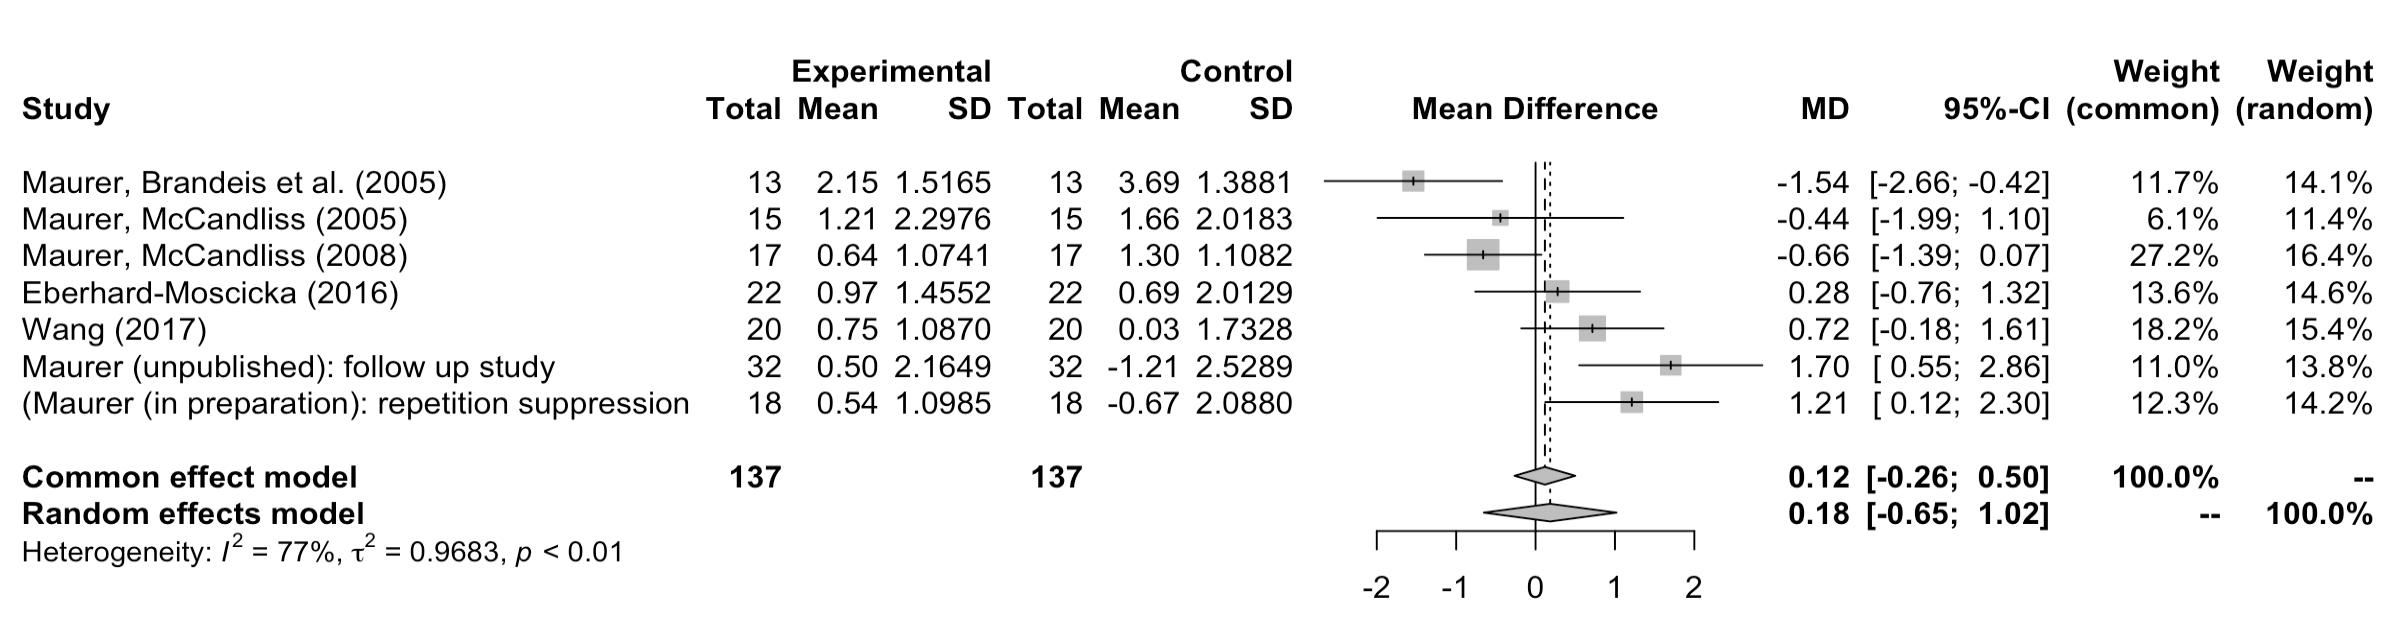
\includegraphics[scale = 0.368]{early_late_N1_PTE.png}
  \caption{Forest plot comparing early and late N1 print tuning effect}
  \label{fig:forest plot 1}
\end{figure}

The Egger’s regression-based test (Egger et al., 1997) did not show the overall publication bias (z =  0.0977, p = 0.9222). In addition, the subgroup analysis displayed much larger p-value within the subgroups (\begin{math}z_{alphabetic} = 0.0187\end{math}, \begin{math}p_{alphabetic} = 0.9851\end{math} and  \begin{math}z_{logographic} = 0.9299\end{math}, \begin{math}p_{logographic} =0.3524)\end{math}, which further proves the symmetries of the selected papers.

\subsection{Visual Similarity \& Moderation Analysis}

As shown in table \ref{table1}, step-wise random-effect moderator analysis (k = 7; estimator: restricted maximum-likelihood estimator) suggested that Model 3 accounts for all variability with least parameters. Therefore it is the model that describes the data the best. The parameters in this model are PC, ON, and DS. @CHECK IF IT'S STROKE OR STROKES@

\begin{table}[h]
\centering
\small % Change font size to small
\begin{tabularx}{\linewidth}{@{}l*{10}{C}@{}}
\toprule
   & \multicolumn{2}{c}{Model 1} & \multicolumn{2}{c}{Model 2} & \multicolumn{2}{c}{Model 3}  & \multicolumn{2}{c}{Model 4}  & \multicolumn{2}{c}{Model 5}  \\ \cmidrule(l){2-11} 
   & estimate      & \textit{p} value     & estimate      & \textit{p} value     & estimate       & \textit{p} value     & estimate       & \textit{p} value     & estimate       & \textit{p} value     \\ \midrule
PC & 2.6583        & 0.7240      & -9.2747       & 0.2875      & -30.8616       & 0.0033      & -30.6845       & 0.0075      & -42.0121       & 0.0211      \\
ON &               &             & 8.7323        & 0.0621      & 20.0045        & 0.0004      & 20.0073        & 0.0004      & 21.1050        & 0.0003      \\
DS &               &             &               &             & -10.1781       & 0.0117      & -10.1129       & 0.0210      & -8.0435        & 0.1139      \\
SS &               &             &               &             &                &             & -0.2076        & 0.9695      & -0.3908        & 0.9427      \\
JC &               &             &               &             &                &             &                &             & -8.9467        & 0.4235      \\ \cmidrule(l){2-11} 
$R^2$  & \multicolumn{2}{c}{0.00\%}  & \multicolumn{2}{c}{37.65\%} & \multicolumn{2}{c}{100.00\%} & \multicolumn{2}{c}{100.00\%} & \multicolumn{2}{c}{100.00\%} \\ \bottomrule
\end{tabularx}
PC: Perimetric Complexity, ON: Object Number, DS: Disconnected Stroke, SS: Stroke Sum, JC: Junction.
\caption{Stepwise Random-Effect Moderator Analysis}
\label{table1}
\end{table}

The random-effect moderator analysis (k = 7; estimator: restricted maximum-likelihood estimator) showed a significant result (QM(df = 2) = 10.8292, p = 0.0045), while the test for residual heterogeneity is not significant (QE (df = 4) = 4.1641, p = 0.3842). 

Additionally, we did a multiple meta-regression analysis involving writing system, and it only raises the p-value rather than lowering it. However, when writing system serves as the only moderator, the random-effect model showed a significant moderation effect (QM(df = 1) = 10.0814, p = 0.0015), while the test for residual heterogeneity is not significant (QE(df = 5) = 3.9813, p = 0.5521).


\subsection{Post-hoc Analysis}

The post-hoc analysis compared word and control conditions separately in the early and late N1 time windows. In the early N1, the random-effect model showed a significant general effect size (MD = -1.0816, p = 0.0007) and no significant heterogeneity (QE (df = 6) = 3.17, p = 0.7871). In the late N1, the random-effect model did not show a significant general effect size (MD = -0.8259, p = 0.1732), but significant heterogeneity was present (QE (df = 6) = 23.24, p = 0.0007). As shown in table \ref{table2} The post-hoc meta-regression found a significant correlation between the difference among studies in the late N1 and 3 visual complexity parameters: PC, ON, and DS.

\begin{table}[h]
\centering
\begin{tabular}{@{}lllllll@{}}
           & estimate & se      & zval    & pval   & ci.lb    & ci.ub    \\ \midrule
intrcpt    & -0.4947  & 0.5010  & -0.9875 & 0.3234 & -1.4766  & 0.4872   \\
PC         & -42.3097 & 14.9328 & -2.8333 & 0.0046 & -71.5773 & -13.0420 \\
obj\_num   & 27.4348  & 7.6107  & 3.6048  & 0.0003 & 12.5181  & 42.3515  \\
disc\_strk & -15.3988 & 5.7660  & -2.6706 & 0.0076 & -26.6999 & -4.0978 

\label{table2}
\end{tabular}
\end{table}

\section{Conclusion}
\subsection{Effect Sizes}

The random-effect model showed significant heterogeneity, supporting our hypothesis that there is a difference in the N1 print tuning effect processing time window among the selected studies. Study 1-3 had a more pronounced early N1 print tuning effect, while no obvious difference was observed in study 4-7. Post-hoc analysis confirmed this finding.

Interestingly, this finding echoes with the results from previous studies since studies using symbols in control conditions found more pronounced word vs. control condition difference in a later time window (Shirahama, 2003; Brem, 2006), while those using false-fonts or unfamiliar words only found an earlier difference (Eberhard-Moscicka et al., 2016; Wang \& Maurer, 2017).

\subsection{Moderation Effect}

The step-wise meta-regression analysis revealed that the 3-parameter model (PC, ON, and DS) best fits the EEG data. This suggests that visual similarity in these aspects of stimuli affects how our brain processes reading. PC and DS are negatively correlated, while ON is positively correlated with the EEG data. This means that an increase in PC and DS shifts the N1 print tuning effect towards early N1, while an increase in ON shifts it towards late N1.

\end{document}